% 第4章第2节：历史信息与适应过程（滤过、自然滤过、适应性、停时）。

\section{历史信息与适应过程}
\label{sec:spp-information}

上一节的有限维分布与路径规律是“事后”的描述：它们把整段记录当作一次给定的结果来看。可是许多问题要求站在某个时刻，只用已经发生的记录作判断：预测下一步时能用哪些读数，什么时候停止监测，下一步的投入能否依赖尚未揭晓的噪声。本节给时间索引加上信息结构。滤过规定每个时刻已经可以判定的事件，适应性检查过程的当前值是否已知，停时则把“何时停下”也纳入同样的要求。第~\ref{chap:discrete-time-stochastic-processes}章与第~\ref{chap:continuous-time-stochastic-processes}章中的Markov性质、鞅性质和随机累计，都相对于这里指定的信息来陈述。

本节的索引集$T$是$\mathbb R$的子集并沿用实数的顺序，典型情形是$T=\mathbb N_0$或$T=[0,\infty)$。

\subsection{滤过与适应性}
\label{sec:spp-filtration-adapted}

\paragraph{信息随时间增长}
回到示例~\ref{ex:spp-three-coins}的三次抛硬币。在时刻$1$，我们只知道第一次的结果；能够判定是否发生的事件，恰好是那些由第一次结果决定的事件，例如“第一次是正面”。在样本空间上看，这相当于把八个结果按第一次的结果分成两块：我们知道$\omega$落在哪一块，却不知道它在块内的位置。到时刻$2$，分块细化为按前两次结果划分的四块；到时刻$3$，每块只剩一个结果。

图~\ref{fig:spp-filtration-layers}把这四层分块从上到下排开，块内数字是随机游走$S_n$在该块上的取值。每一层的块都是上一层某一块的再分割，因为新的记录只会增加、不会抹去已知的结果。另一个值得注意的事实是：$S_n$在第$n$层的每一块内取常数，所以到时刻$n$为止的记录足以确定$S_n$；而$S_3$在第$2$层的块内并不是常数，例如$\mathrm{HH}*$块中$S_3$可能是$3$也可能是$1$，在时刻$2$还不能确定。

\begin{figure}[htbp]
  \centering
  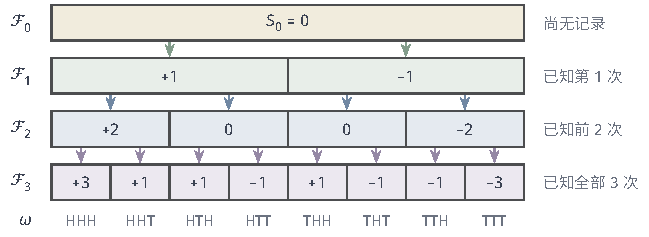
\includegraphics[width=110mm]{figures/03-optimization-evolution-and-signals/02-processes-and-trajectory-evolution/tikz/spp-filtration-layers/figure.pdf}
  \caption{三次抛硬币的自然滤过。最下一行是八个等可能的结果$\omega$；第$n$行把它们按前$n$次结果分块，每一块是$\mathcal F_n$中不可再分的事件，$\mathcal F_n$由这些块的全部并组成。块内数字是随机游走$S_n$（正面$+1$、反面$-1$）在该块上的取值；箭头表示每一层都是上一层的细分。}
  \label{fig:spp-filtration-layers}
\end{figure}

\paragraph{滤过与自然滤过}
在一般概率空间上，“时刻$t$能够判定的事件”组成一个子$\sigma$代数，记作$\mathcal F_t$。信息只增不减，于是得到一列递增的子$\sigma$代数。

\begin{definition}[滤过与自然滤过]
\label{def:spp-filtration}
设$(\Omega,\mathcal F,\mathbb P)$是概率空间，$T\subseteq\mathbb R$。一族子$\sigma$代数$(\mathcal F_t)_{t\in T}$若满足
\[
  \mathcal F_s\subseteq\mathcal F_t\subseteq\mathcal F,\qquad s,t\in T,\ s\le t,
\]
就称为\term{滤过}（filtration），$(\Omega,\mathcal F,(\mathcal F_t)_{t\in T},\mathbb P)$称为带滤过的概率空间。对随机过程$X=(X_t)_{t\in T}$，
\[
  \mathcal F^X_t=\sigma(X_s:\ s\in T,\ s\le t)
\]
是由截至时刻$t$的记录生成的$\sigma$代数，$(\mathcal F^X_t)_{t\in T}$称为$X$的\term{自然滤过}（natural filtration）。
\end{definition}

滤过描述的是“谁知道什么”，不一定由所研究的过程本身生成。一个观测者可能从一开始就掌握某个初始信息，也可能同时看到另一路信号；这时他的信息族比$X$的自然滤过更大。同一个过程可以相对于不同的滤过研究，后面会看到，结论可能因此改变。

\paragraph{适应过程}
有了滤过，就可以说一个随机量“在时刻$t$已经可知”：它关于$\mathcal F_t$可测，意味着对每个可测集$B$，事件“它落在$B$中”在时刻$t$已经可以判定。

\begin{definition}[适应过程]
\label{def:spp-adapted}
若对每个$t\in T$，$X_t$关于$\mathcal F_t$可测，就称过程$X=(X_t)_{t\in T}$适应于滤过$(\mathcal F_t)_{t\in T}$，也称$X$是\term{适应过程}（adapted process）。
\end{definition}

每个过程都适应于自己的自然滤过，而且自然滤过是使它适应的最小滤过：若$X$适应于$(\mathcal G_t)$，则对$s\le t$有$X_s$关于$\mathcal G_s\subseteq\mathcal G_t$可测，所以生成的$\sigma$代数$\mathcal F^X_t\subseteq\mathcal G_t$。在有限样本空间上，若$\mathcal F_n$由一个有限分块生成，那么$X_n$关于$\mathcal F_n$可测，当且仅当$X_n$在每一块上取常数：每个事件$\{X_n=x\}$都必须是若干整块的并。图~\ref{fig:spp-filtration-layers}中$S_n$在第$n$层每块上为常数，正是适应性的直观形态；而$S_{n+1}$通常不在第$n$层的块上取常数，所以“下一时刻的位置”这个过程$(S_{n+1})_n$不适应于自然滤过。

\begin{example}[按块平均的预测]
\label{ex:spp-block-average}
在图~\ref{fig:spp-filtration-layers}的有限样本空间上，给定$\mathcal F_n$的条件期望就是在第$n$层的每一块内对等可能结果取平均。例如在时刻$1$预测$S_3$：$\mathrm H**$块中$S_3$的四个值为$3,1,1,-1$，平均为$1$；$\mathrm T**$块中为$1,-1,-1,-3$，平均为$-1$。所以$\mathbb E[S_3\mid\mathcal F_1]=S_1$。同样地，在第$2$层的$\mathrm{HH}*$块中$S_3$取$3$或$1$，平均为$2=S_2$。在这个模型中，用截至当前的记录预测未来位置，最好的均方预测就是当前位置；把第$1$层的块平均再在第$0$层平均，得到$\mathbb ES_3=0$，这正是塔式性质在分块上的样子：先在细块内平均，再在粗块内平均，等于直接在粗块内平均。
\end{example}

\paragraph{同一过程，不同信息}
下面的例子说明，同一个过程在两种滤过下给出不同的预测，二者之间的关系由条件期望的塔式性质刻画。

\begin{example}[共享背景下的两个观测者]
\label{ex:spp-two-observers}
沿用第~\ref{sec:spp-index-state-space}小节的共享背景读数$X_n=\Theta+\varepsilon_n$，$\Theta\sim\mathcal N(0,\tau^2)$，噪声$\varepsilon_n$独立服从$\mathcal N(0,\sigma^2)$且与$\Theta$独立。观测者甲只看到读数，信息为自然滤过$\mathcal F_n=\sigma(X_1,\ldots,X_n)$；观测者乙事先知道$\Theta$，信息为$\mathcal G_n=\sigma(\Theta,X_1,\ldots,X_n)$。读数过程同时适应于这两个滤过，并且$\mathcal F_n\subseteq\mathcal G_n$。

对乙而言，$\varepsilon_{n+1}$与$\mathcal G_n$独立且均值为零，所以
\[
  \mathbb E[X_{n+1}\mid\mathcal G_n]=\Theta+\mathbb E[\varepsilon_{n+1}\mid\mathcal G_n]=\Theta .
\]
对甲而言，$\varepsilon_{n+1}$同样与$\mathcal F_n$独立，于是$\mathbb E[X_{n+1}\mid\mathcal F_n]=\mathbb E[\Theta\mid\mathcal F_n]$。为了算出它，令$\bar X_n=\frac1n\sum_{i=1}^nX_i$，$c=n\tau^2/(n\tau^2+\sigma^2)$，并考虑残差$R=\Theta-c\bar X_n$。直接计算
\[
  \operatorname{Cov}(R,X_i)=\tau^2-c\Bigl(\tau^2+\frac{\sigma^2}{n}\Bigr)=0,\qquad i=1,\ldots,n .
\]
$(R,X_1,\ldots,X_n)$是独立高斯变量的线性组合，因而联合高斯；联合高斯向量中不相关的分量相互独立，所以$R$与$\mathcal F_n$独立，$\mathbb E[R\mid\mathcal F_n]=\mathbb ER=0$。于是
\[
  \mathbb E[X_{n+1}\mid\mathcal F_n]=c\,\bar X_n=\frac{n\tau^2}{n\tau^2+\sigma^2}\,\bar X_n .
\]
甲把读数平均值向零收缩，因为他不知道这个平均值中有多少来自$\Theta$、多少来自噪声；读数越多，收缩系数越接近$1$。

两个预测满足塔式性质$\mathbb E\bigl[\mathbb E[X_{n+1}\mid\mathcal G_n]\bigm|\mathcal F_n\bigr]=\mathbb E[X_{n+1}\mid\mathcal F_n]$：把乙的预测$\Theta$按甲的信息再平均一次，正好得到甲的预测。预测误差也可以直接比较。乙的均方误差是$\mathbb E\varepsilon_{n+1}^2=\sigma^2$；甲的误差$X_{n+1}-c\bar X_n=R+\varepsilon_{n+1}$，均方误差为
\[
  \sigma^2+\operatorname{Var}(R)=\sigma^2+\frac{\tau^2\sigma^2}{n\tau^2+\sigma^2},
\]
其中$\operatorname{Var}(R)=\tau^2-c^2(\tau^2+\sigma^2/n)=\tau^2(1-c)$。取$\tau=\sigma=1$、$n=4$，甲的预测为$0.8\bar X_4$，均方误差$1.2$；乙的预测为$\Theta$，均方误差$1$。信息越多，最优均方预测的误差越小，这是塔式性质下条件方差分解的一个具体实例。
\end{example}

\paragraph{性质要相对于滤过说明}
滤过的选择不仅影响预测的数值，也影响过程是否具有某种性质。第~\ref{chap:discrete-time-stochastic-processes}章将正式定义鞅与Markov性质；这里只用它们的直观含义看一个对照。设$\xi_1,\xi_2,\ldots$独立，等概率取$\pm1$，$S_0=0$，$S_n=\xi_1+\cdots+\xi_n$。相对于自然滤过$\mathcal F_n=\sigma(\xi_1,\ldots,\xi_n)$，下一步的条件平均不变：
\[
  \mathbb E[S_{n+1}\mid\mathcal F_n]=S_n+\mathbb E\xi_{n+1}=S_n ,
\]
这正是“公平博弈”的性质。现在设想一个提前一步知道结果的观测者，他的信息为$\mathcal H_n=\sigma(\xi_1,\ldots,\xi_{n+1})$。$S$仍然适应于$(\mathcal H_n)$，但
\[
  \mathbb E[S_{n+1}\mid\mathcal H_n]=S_{n+1}\ne S_n ,
\]
对这个观测者而言，博弈不再公平。因此，“$S$是鞅”这句话必须带上滤过才有意义。

Markov性质也一样。在示例~\ref{ex:spp-two-observers}中，乙给定$\mathcal G_n$时下一读数的条件分布是$\mathcal N(\Theta,\sigma^2)$，只通过$\Theta$依赖已有信息；甲给定$\mathcal F_n$时，下一读数的条件分布依赖全部读数的平均值$\bar X_n$，单凭当前读数$X_n$并不足够。若把$(n,\bar X_n)$一并放进状态，甲面对的就是一个只依赖当前状态的递推。状态是否“足够”同样是相对于信息结构而言的，第~\ref{chap:discrete-time-stochastic-processes}章将在一般条件下讨论这一点。

\subsection{随机时刻与停止时刻}
\label{sec:spp-stopping-times}

\paragraph{何时停下由记录决定}
监测常常在读数第一次越过阈值时结束，赌徒可能在赢够一定数额时离场，迭代算法在误差指标首次低于容差时终止。这些停止时刻都是随机的：不同的实验结果在不同的时刻停下。随机时刻是取值于$T\cup\{\infty\}$的映射$\tau:\Omega\to T\cup\{\infty\}$，$\tau(\omega)=\infty$表示永不停止。一条停止规则能够实际执行，必须满足一个要求：在每个时刻$t$，只凭截至$t$的记录就能判断是否已经停下。

\paragraph{停时的定义}
把这个要求写成可测性条件，就得到下面的定义。

\begin{definition}[停时]
\label{def:spp-stopping-time}
设$(\mathcal F_t)_{t\in T}$是滤过。随机时刻$\tau:\Omega\to T\cup\{\infty\}$若对每个$t\in T$满足
\[
  \{\tau\le t\}\in\mathcal F_t ,
\]
就称为相对于该滤过的\term{停时}（stopping time），也称停止时刻。
\end{definition}

离散时间$T=\mathbb N_0$时，这个条件等价于对每个$n$有$\{\tau=n\}\in\mathcal F_n$。若$\{\tau\le n\}\in\mathcal F_n$对每个$n$成立，则$\{\tau=n\}=\{\tau\le n\}\setminus\{\tau\le n-1\}$，后一个集合属于$\mathcal F_{n-1}\subseteq\mathcal F_n$；反之，$\{\tau\le n\}=\bigcup_{k=0}^n\{\tau=k\}$，每一项属于$\mathcal F_k\subseteq\mathcal F_n$。离散情形下“现在是否恰好停下”与“现在是否已经停下”可以互相判定；连续时间中单点时刻的事件往往概率为零，定义因此采用$\{\tau\le t\}$。

常数时刻$\tau\equiv t_0$是停时，因为$\{\tau\le t\}$是$\varnothing$或$\Omega$。若$\tau,\sigma$都是停时，则$\tau\wedge\sigma=\min(\tau,\sigma)$与$\tau\vee\sigma=\max(\tau,\sigma)$也是停时：
\begin{gather*}
  \{\tau\wedge\sigma\le t\}=\{\tau\le t\}\cup\{\sigma\le t\},\\
  \{\tau\vee\sigma\le t\}=\{\tau\le t\}\cap\{\sigma\le t\},
\end{gather*}
右边都属于$\mathcal F_t$。特别地，$\tau\wedge n$是一个不超过$n$的停时，第~\ref{chap:discrete-time-stochastic-processes}章常用它把可能无界的停时截断。

\paragraph{首次命中与全程最高点}
最常见的停时是首次命中时刻。设$S$是随机游走，取整数阈值$a>0$，令
\[
  \tau_a=\inf\{n\ge0:\ S_n\ge a\},\qquad \inf\varnothing=\infty .
\]
对每个$n$，
\[
  \{\tau_a\le n\}=\bigcup_{k=0}^n\{S_k\ge a\}\in\mathcal F_n ,
\]
因为每个$S_k$（$k\le n$）关于$\mathcal F_k\subseteq\mathcal F_n$可测。同样的论证表明：若$X$适应于$(\mathcal F_n)$，$B$是可测集，则首次进入时刻$\inf\{n:\ X_n\in B\}$是停时。图~\ref{fig:spp-stopping-vs-peak}(a)中，路径在$n=7$第一次达到阈值$3$，停止的决定当场就能做出，之后的灰色部分与判断无关。

与之对照，考虑在$\{0,1,\ldots,N\}$上首次达到全程最大值的时刻$\sigma=\min\{n\le N:\ S_n=\max_{k\le N}S_k\}$。取$N=2$并逐一列出四种结果：$\mathrm{HH}$时路径为$0,1,2$，$\sigma=2$；$\mathrm{HT}$时为$0,1,0$，$\sigma=1$；$\mathrm{TH}$时为$0,-1,0$，最大值$0$首次出现在$n=0$，$\sigma=0$；$\mathrm{TT}$时$\sigma=0$。于是$\{\sigma=1\}=\{\xi_1=+1,\ \xi_2=-1\}$，它依赖第二次的结果，不属于只含$\varnothing$、$\{\xi_1=+1\}$、$\{\xi_1=-1\}$与$\Omega$的$\mathcal F_1$。所以$\sigma$不是停时。图~\ref{fig:spp-stopping-vs-peak}(b)显示了一般原因：到$n=6$为止，两条路径的历史完全相同，$n=5$是迄今的最高点；它是否是全程最高点，取决于之后走低还是走高。

\begin{figure}[htbp]
  \centering
  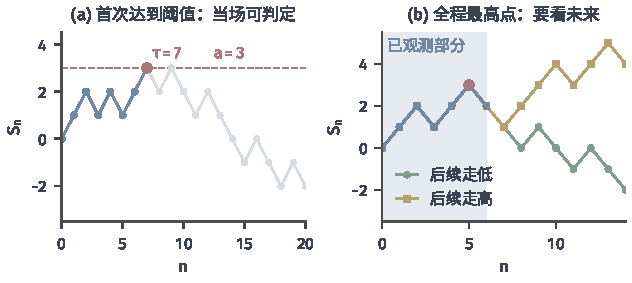
\includegraphics[width=107mm]{figures/03-optimization-evolution-and-signals/02-processes-and-trajectory-evolution/matplotlib/spp-stopping-vs-peak/figure.pdf}
  \caption{停时与非停时。两图均为步长$\pm1$的教学路径。(a)首次达到阈值$a=3$的时刻$\tau=7$（红点）：是否停止只需看到当前为止的蓝色部分。(b)两条路径在浅蓝区域（$n\le6$）内完全相同，$n=5$（红点）是迄今最高点；绿色延续中它仍是全程最高点，黄色延续中则不是。“全程最高点的时刻”要看未来才能判定。}
  \label{fig:spp-stopping-vs-peak}
\end{figure}

\paragraph{定义不提供期望等式}
停时的定义只保证停止规则不偷看未来，并不保证停止后各种平均关系依然成立。下面的倍投策略是标准的警示。

\begin{example}[倍投策略]
\label{ex:spp-doubling}
设$\xi_1,\xi_2,\ldots$独立，等概率取$\pm1$，代表一枚公平硬币。赌徒第$k$轮押注$2^{k-1}$，累计盈亏为$M_0=0$，$M_n=\sum_{k=1}^n2^{k-1}\xi_k$。每轮押注在开局前已经确定，硬币公平，所以$\mathbb E[M_{n+1}\mid\mathcal F_n]=M_n+2^n\mathbb E\xi_{n+1}=M_n$，对每个固定的$n$都有$\mathbb EM_n=0$。赌徒在第一次赢时离场：$\tau=\min\{k:\ \xi_k=+1\}$。它是首次命中时刻，因而是停时；又$\mathbb P(\tau>n)=2^{-n}$，所以$\tau<\infty$几乎必然成立。

在离场时刻，前$\tau-1$轮共输$1+2+\cdots+2^{\tau-2}=2^{\tau-1}-1$，第$\tau$轮赢$2^{\tau-1}$，故$M_\tau=1$恒成立，$\mathbb EM_\tau=1\ne0=\mathbb EM_0$。截断后的情形则不同：若$\tau\le n$，则$M_{\tau\wedge n}=1$；若$\tau>n$，则前$n$轮全输，$M_{\tau\wedge n}=-(2^n-1)$。于是
\[
  \mathbb EM_{\tau\wedge n}=(1-2^{-n})\cdot1+2^{-n}\cdot\bigl(-(2^n-1)\bigr)=0 .
\]
$M_{\tau\wedge n}$几乎必然收敛到$M_\tau=1$，期望却一直是$0$：概率$2^{-n}$的巨额亏损恰好抵消了其余情形的收益，在极限中消失。
\end{example}

这个例子说明，停时之后的期望等式需要额外条件来排除“小概率、大损失”的情形。第~\ref{chap:discrete-time-stochastic-processes}章在离散时间中建立可选停止定理及其条件，并用停时陈述强Markov性质。连续时间中，即使是首次命中时刻也需要额外的路径与滤过条件才能保证是停时，例如路径右连续、滤过满足适当的右连续性；这些条件及相应的可积性要求由第~\ref{chap:continuous-time-stochastic-processes}章补充。
